% CVPR 2026 Paper Template; based on the supplied official author kit.
\documentclass[10pt,twocolumn,letterpaper]{article}

\usepackage[pagenumbers]{cvpr}
\usepackage{times}
\usepackage{epsfig}
\usepackage{graphicx}
\usepackage{amsmath}
\usepackage{amssymb}
\usepackage{booktabs}
\usepackage{multirow}
\usepackage{microtype}
\usepackage{xcolor}
\usepackage{url}

\definecolor{cvprblue}{rgb}{0.21,0.49,0.74}
\usepackage[pagebackref,breaklinks,colorlinks,allcolors=cvprblue]{hyperref}

\def\paperID{COMP9517}
\def\confName{CVPR}
\def\confYear{2026}

\title{Fine-Grained Species Recognition on iNaturalist-2021:\\
Classical Features, ResNet-18, Transfer Learning, and Grad-CAM}

\author{Suraj Pratap Singh\\
Sydney, Australia\\
{\tt\small suraj\_pratap.singh@student.unsw.edu.au}}

\begin{document}
\maketitle

\begin{abstract}
In this project, we classify 500 iNaturalist species using a balanced set of 30,000 images.  We tried two different approaches: handcrafted image features with classical classifiers, and ResNet-18 based deep-learning models.  For the classical approach, SIFT with bag-of-visual-words and a linear SVM gave the best result, but its top-1 accuracy was only 3.42\%.  ResNet-18 trained from scratch achieved 41.98\%.  When we started from ImageNet pretrained weights and fine-tuned the model, top-1 accuracy increased to 66.02\%, top-5 accuracy to 83.30\%, and macro-F1 to 65.76\%.  We also compared HOG, HSV, HOG+HSV, different SIFT vocabulary sizes, and two classical classifiers.  The report includes training curves, confusion examples, failure cases, and Grad-CAM visualisations.  The results show that transfer learning helps a lot when there are only 40 training images per class, although there is still clear overfitting.
\end{abstract}

\section{Introduction}
Fine-grained image classification means that the classes look quite similar to each other.  In our case, the model has to tell apart 500 species.  A small change in colour, leaf shape, wing pattern, or texture can matter, but the images also have different poses, lighting, camera quality, and backgrounds.  iNaturalist is useful for this because it contains real observations taken in uncontrolled conditions, not studio images \cite{vanhorn2021benchmarking}.  In our selected dataset, every class has only 40 training images, which makes the task more difficult.

Instead of using only one model, we compared old-style computer vision methods with deep learning.  For the first group, we used SIFT \cite{lowe2004distinctive}, bag-of-visual-words (BoVW) \cite{csurka2004visual}, HOG \cite{dalal2005histograms}, HSV colour histograms, linear classifiers, and a random forest.  For the deep-learning part, we used the same ResNet-18 network \cite{he2016deep} in two ways: training it from scratch and fine-tuning it from ImageNet weights \cite{deng2009imagenet}.  We also used Grad-CAM \cite{selvaraju2017grad} to see which parts of an image influenced a prediction.

The main things we did in this project are:
\begin{itemize}
    \item make a fixed balanced split with 20,000 training, 5,000 validation, and 5,000 test images;
    \item run classical and deep-learning pipelines on the same split and compare them using the same metrics;
    \item test different handcrafted features, SIFT vocabulary sizes, classifiers, and ResNet initialisation methods; and
    \item analyse training behaviour, errors, timing, and Grad-CAM outputs.
\end{itemize}

\section{Literature Review}
\subsection{Handcrafted visual representations}
Before CNNs became common, image classification was usually split into feature extraction, feature aggregation, and classification.  SIFT finds keypoints and describes the local gradients around them.  It was designed to be fairly stable under scale, rotation, and moderate lighting changes \cite{lowe2004distinctive}.  Since an image can have a different number of SIFT keypoints, BoVW maps them to a learned visual vocabulary and stores the counts as one fixed-length histogram \cite{csurka2004visual}.  This is easy to train, but it also loses the original position of the keypoints, which can be important when two species have similar local textures.

HOG stores the direction of image gradients over a fixed grid \cite{dalal2005histograms}.  It can capture edges, shape, and texture, but it can struggle when the object moves a lot in the image.  HSV histograms give simple colour information, but they do not say where the colour appears.  We used these features because they are standard and give understandable baselines.  A linear SVM is a practical classifier for large feature vectors, while a random forest gives us one nonlinear comparison.  So, the classical experiments do not depend on only one feature or one classifier.

\subsection{Deep and transfer learning for fine-grained recognition}
CNNs learn the image features directly instead of using manually designed descriptors.  ResNet adds shortcut connections, making deep networks easier to train \cite{he2016deep}.  We selected ResNet-18 because it is not too large and it can be trained repeatedly with our available hardware.  Fine-grained recognition can benefit from focusing on small discriminative parts, as shown by bilinear CNN methods \cite{lin2015bilinear}.  We kept the network simple in this project so that the comparison between scratch training and pretrained training stays clear.

ImageNet pretraining gives the network a starting point from a much bigger image dataset \cite{deng2009imagenet}.  Earlier layers often learn general edges and textures, while later layers are more task-specific.  This is why replacing the final classifier and then fine-tuning the full network is a common transfer-learning method \cite{yosinski2014transferable}.  However, good ImageNet performance does not automatically mean good target-task performance \cite{kornblith2019better}, so we still evaluated it properly on our own validation and test splits.  This is important here because each class has very limited training data.

The iNaturalist images have changes in scale, pose, background, and image quality \cite{vanhorn2021benchmarking}.  We used random crops, flips, colour jitter, rotation, weight decay, and label smoothing to handle some of this variation.  Label smoothing can reduce overconfident predictions, although it does not always help every task \cite{muller2019label}.  Grad-CAM uses gradients from the class score to show which convolutional regions affected a prediction \cite{selvaraju2017grad}.  It is useful for checking the model, but it does not prove that the model is reasoning correctly.

\section{Dataset and Experimental Protocol}
\subsection{Balanced iNaturalist subset}
We prepared the selected iNaturalist archive using a notebook that creates one fixed mapping from class names to class indices.  The final data has 500 species and 60 images per species: 40 for training, 10 for validation, and 10 for testing.  This gives 30,000 images in total.  We used seed 42.  Images that came from the same source identifier were kept in the same split so that near-duplicate images do not leak into validation or test.  Before training, we checked paths, labels, class counts, split sizes, and overlap between the manifests.

We used validation data for choosing checkpoints and hyperparameters.  The test data was kept for final evaluation.  Since each class has the same number of test images, overall accuracy, top-1 accuracy, balanced accuracy, and macro recall become the same number here.  We still saved all of them so that the evaluation is complete and easy to compare across methods.

\subsection{Metrics}
For an image $i$ with true class $y_i$, top-$k$ accuracy checks whether the correct class is in the top $k$ model predictions.  We report top-1 and top-5 accuracy, macro precision, macro recall, and macro-F1.  For $C=500$ classes,
\begin{equation}
 F_{1,\mathrm{macro}}=\frac{1}{C}\sum_{c=1}^{C}
 \frac{2P_cR_c}{P_c+R_c}.
\end{equation}
Macro averaging gives every class equal importance.  This matters in general even though our selected test split is balanced.  We also saved full test predictions, confusion matrices, commonly confused class pairs, inference time, and throughput.

\section{Methods}
\subsection{SIFT bag-of-visual-words}
For the main traditional method, we first convert each image to grayscale and resize it only if its longest side is more than 200 pixels.  OpenCV SIFT then gives 128-dimensional descriptors around detected keypoints.  We sampled at most 100,000 training descriptors using seed 42 and trained MiniBatchKMeans ($n_{\mathrm{init}}=1$, batch size 1,000) to make $K$ visual words.  Every image is represented by an $\ell_2$-normalised histogram of those words.

We fit the standard scaler only on training histograms.  Our main classifier is \texttt{SGDClassifier} with hinge loss, $\alpha=10^{-4}$, tolerance $10^{-3}$, and at most 1,000 iterations.  This works like a linear SVM trained using stochastic optimisation.  The main result uses $K=200$, and we also tested $K\in\{50,100,200,400\}$.  On the same $K=200$ features, we trained a random forest with 150 trees and maximum depth 25 to check whether a nonlinear classifier helps.

\subsection{HOG and HSV descriptors}
For another handcrafted experiment, we resize RGB images to $128\times128$.  HOG is calculated on luminance using nine orientations, $8\times8$ pixel cells, $2\times2$ cell blocks, L2-Hys normalisation, and square-root intensity compression.  This gives 8,100 features.  HSV uses global histograms with 32 hue bins, 16 saturation bins, and 16 value bins, giving 64 features.  Combining both gives 8,164 features.

We standardise each feature set and train an SGD hinge-loss classifier for ten epochs.  We tried $C\in\{0.01,0.1,1,10\}$ and selected using validation macro-F1.  These runs help us see whether shape features, colour features, or both together are useful for this dataset.

\subsection{ResNet-18 from scratch}
For the scratch model, we replace the ResNet-18 output layer with a 500-class layer and start with random weights.  Training images use random resized crops to $224\times224$ (scale 0.65--1.0), horizontal flips, colour jitter of 0.2, and rotations up to $10^{\circ}$.  Validation and test images are resized to 256 pixels and centre-cropped to 224.  We use ImageNet mean and standard deviation for normalisation.

We train it with cross-entropy loss with label smoothing 0.1, SGD learning rate 0.05, momentum 0.9, weight decay $10^{-4}$, and batch size 64.  The learning rate follows a cosine schedule down to $10^{-5}$.  The maximum was 60 epochs and early stopping patience was 12.  We saved the checkpoint with the lowest validation loss.  Mixed precision was enabled when the device supported it.

\subsection{ImageNet transfer learning}
The pretrained model uses the same ResNet-18, transforms, labels, and data split, but starts with ImageNet-1K weights.  We replaced the last layer and fine-tuned the whole model instead of freezing the backbone.  We used AdamW \cite{loshchilov2019decoupled} with learning rate $3\times10^{-4}$, weight decay $10^{-4}$, label smoothing 0.1, and cosine decay to $10^{-6}$.  This run had a maximum of 30 epochs and early stopping patience 8.  So the main difference is that the pretrained model starts with useful visual features and uses a smaller fine-tuning learning rate.

\subsection{Grad-CAM interpretation}
For the trained scratch model, Grad-CAM hooks the final residual stage, \texttt{layer4[-1]}.  Given class score $s^c$ and activation map $A^k$, channel importance is
\begin{equation}
 \alpha_k^c=\frac{1}{Z}\sum_{u,v}\frac{\partial s^c}{\partial A_{uv}^k},\qquad
 L^c=\mathrm{ReLU}\left(\sum_k\alpha_k^cA^k\right).
\end{equation}
We resize the heatmap and put it on top of the original image.  We generated maps for correct predictions, confident wrong predictions, and images from the most common confusion pair.  Grad-CAM is only for checking the model: a good-looking heatmap does not prove that the model is using the right biological features.

\section{Experimental Results}
\subsection{Experimental setup}
All methods use the same seed-42 manifests and the same 500-class mapping.  We ran the neural models using PyTorch on Apple MPS.  The classical methods use OpenCV and scikit-learn on CPU, and feature caches make reruns faster.  We used validation data to select neural checkpoints, SIFT settings, and HOG/HSV regularisation.  The final numbers come from the untouched 5,000-image test set.  Table~\ref{tab:hyperparameters} lists the important deep-learning settings; the handcrafted settings are given in the Methods section.

\begin{table}[t]
\centering
\caption{Main ResNet-18 training hyperparameters.  Both runs use $224\times224$ input, batch size 64, weight decay $10^{-4}$, label smoothing 0.1, cosine scheduling, and best-validation-loss selection.}
\label{tab:hyperparameters}
\small
\setlength{\tabcolsep}{4.2pt}
\begin{tabular}{lrr}
\toprule
Setting & Scratch & ImageNet \\
\midrule
Epoch budget & 60 & 30 \\
Optimizer & SGD & AdamW \\
Initial learning rate & 0.05 & $3\times10^{-4}$ \\
Minimum learning rate & $10^{-5}$ & $10^{-6}$ \\
Momentum & 0.9 & -- \\
Early-stop patience & 12 & 8 \\
Best epoch & 53 & 22 \\
\bottomrule
\end{tabular}
\end{table}

\subsection{Overall comparison}
Table~\ref{tab:overall} gives the final test results.  Random guessing in 500 classes would be only 0.20\% top-1 and 1.00\% top-5.  All our methods beat this, but the difference between classical and deep learning is very large.  The best traditional model, SIFT--BoVW with the SGD linear SVM, gets 3.42\% top-1 and 11.06\% top-5.  Scratch ResNet-18 reaches 41.98\% top-1.  The pretrained ResNet-18 is the best model with 66.02\% top-1, 83.30\% top-5, and 65.76\% macro-F1.

\begin{table*}[t]
\centering
\caption{Test performance on 5,000 images from 500 balanced classes.  Values are percentages.  ``SIFT--RF'' and ``SIFT--SGD'' use the same 200-word BoVW input.  Best results are bold.}
\label{tab:overall}
\small
\setlength{\tabcolsep}{5.3pt}
\begin{tabular}{lrrrrrr}
\toprule
Method & Top-1 & Top-5 & Balanced acc. & Macro precision & Macro recall & Macro-F1 \\
\midrule
HSV + SGD & 1.94 & 6.96 & 1.94 & 1.82 & 1.94 & 1.58 \\
HOG + SGD & 1.96 & 6.20 & 1.96 & 2.11 & 1.96 & 1.78 \\
HOG+HSV + SGD & 1.72 & 6.76 & 1.72 & 1.84 & 1.72 & 1.67 \\
SIFT--BoVW--RF & 2.04 & 5.74 & 2.04 & 1.49 & 2.04 & 1.60 \\
SIFT--BoVW--SGD & 3.42 & 11.06 & 3.42 & 3.36 & 3.42 & 2.75 \\
ResNet-18, scratch & 41.98 & 63.46 & 41.98 & 42.42 & 41.98 & 41.28 \\
ResNet-18, ImageNet & \textbf{66.02} & \textbf{83.30} & \textbf{66.02} & \textbf{67.75} & \textbf{66.02} & \textbf{65.76} \\
\bottomrule
\end{tabular}
\end{table*}

Compared with scratch training, pretraining improves top-1 by 24.04 points, top-5 by 19.84 points, and macro-F1 by 24.48 points.  This is a big improvement.  The pretrained model already has useful knowledge about edges, texture, shape, and object parts, which is hard to learn from only 40 images per species.

\begin{figure*}[t]
    \centering
    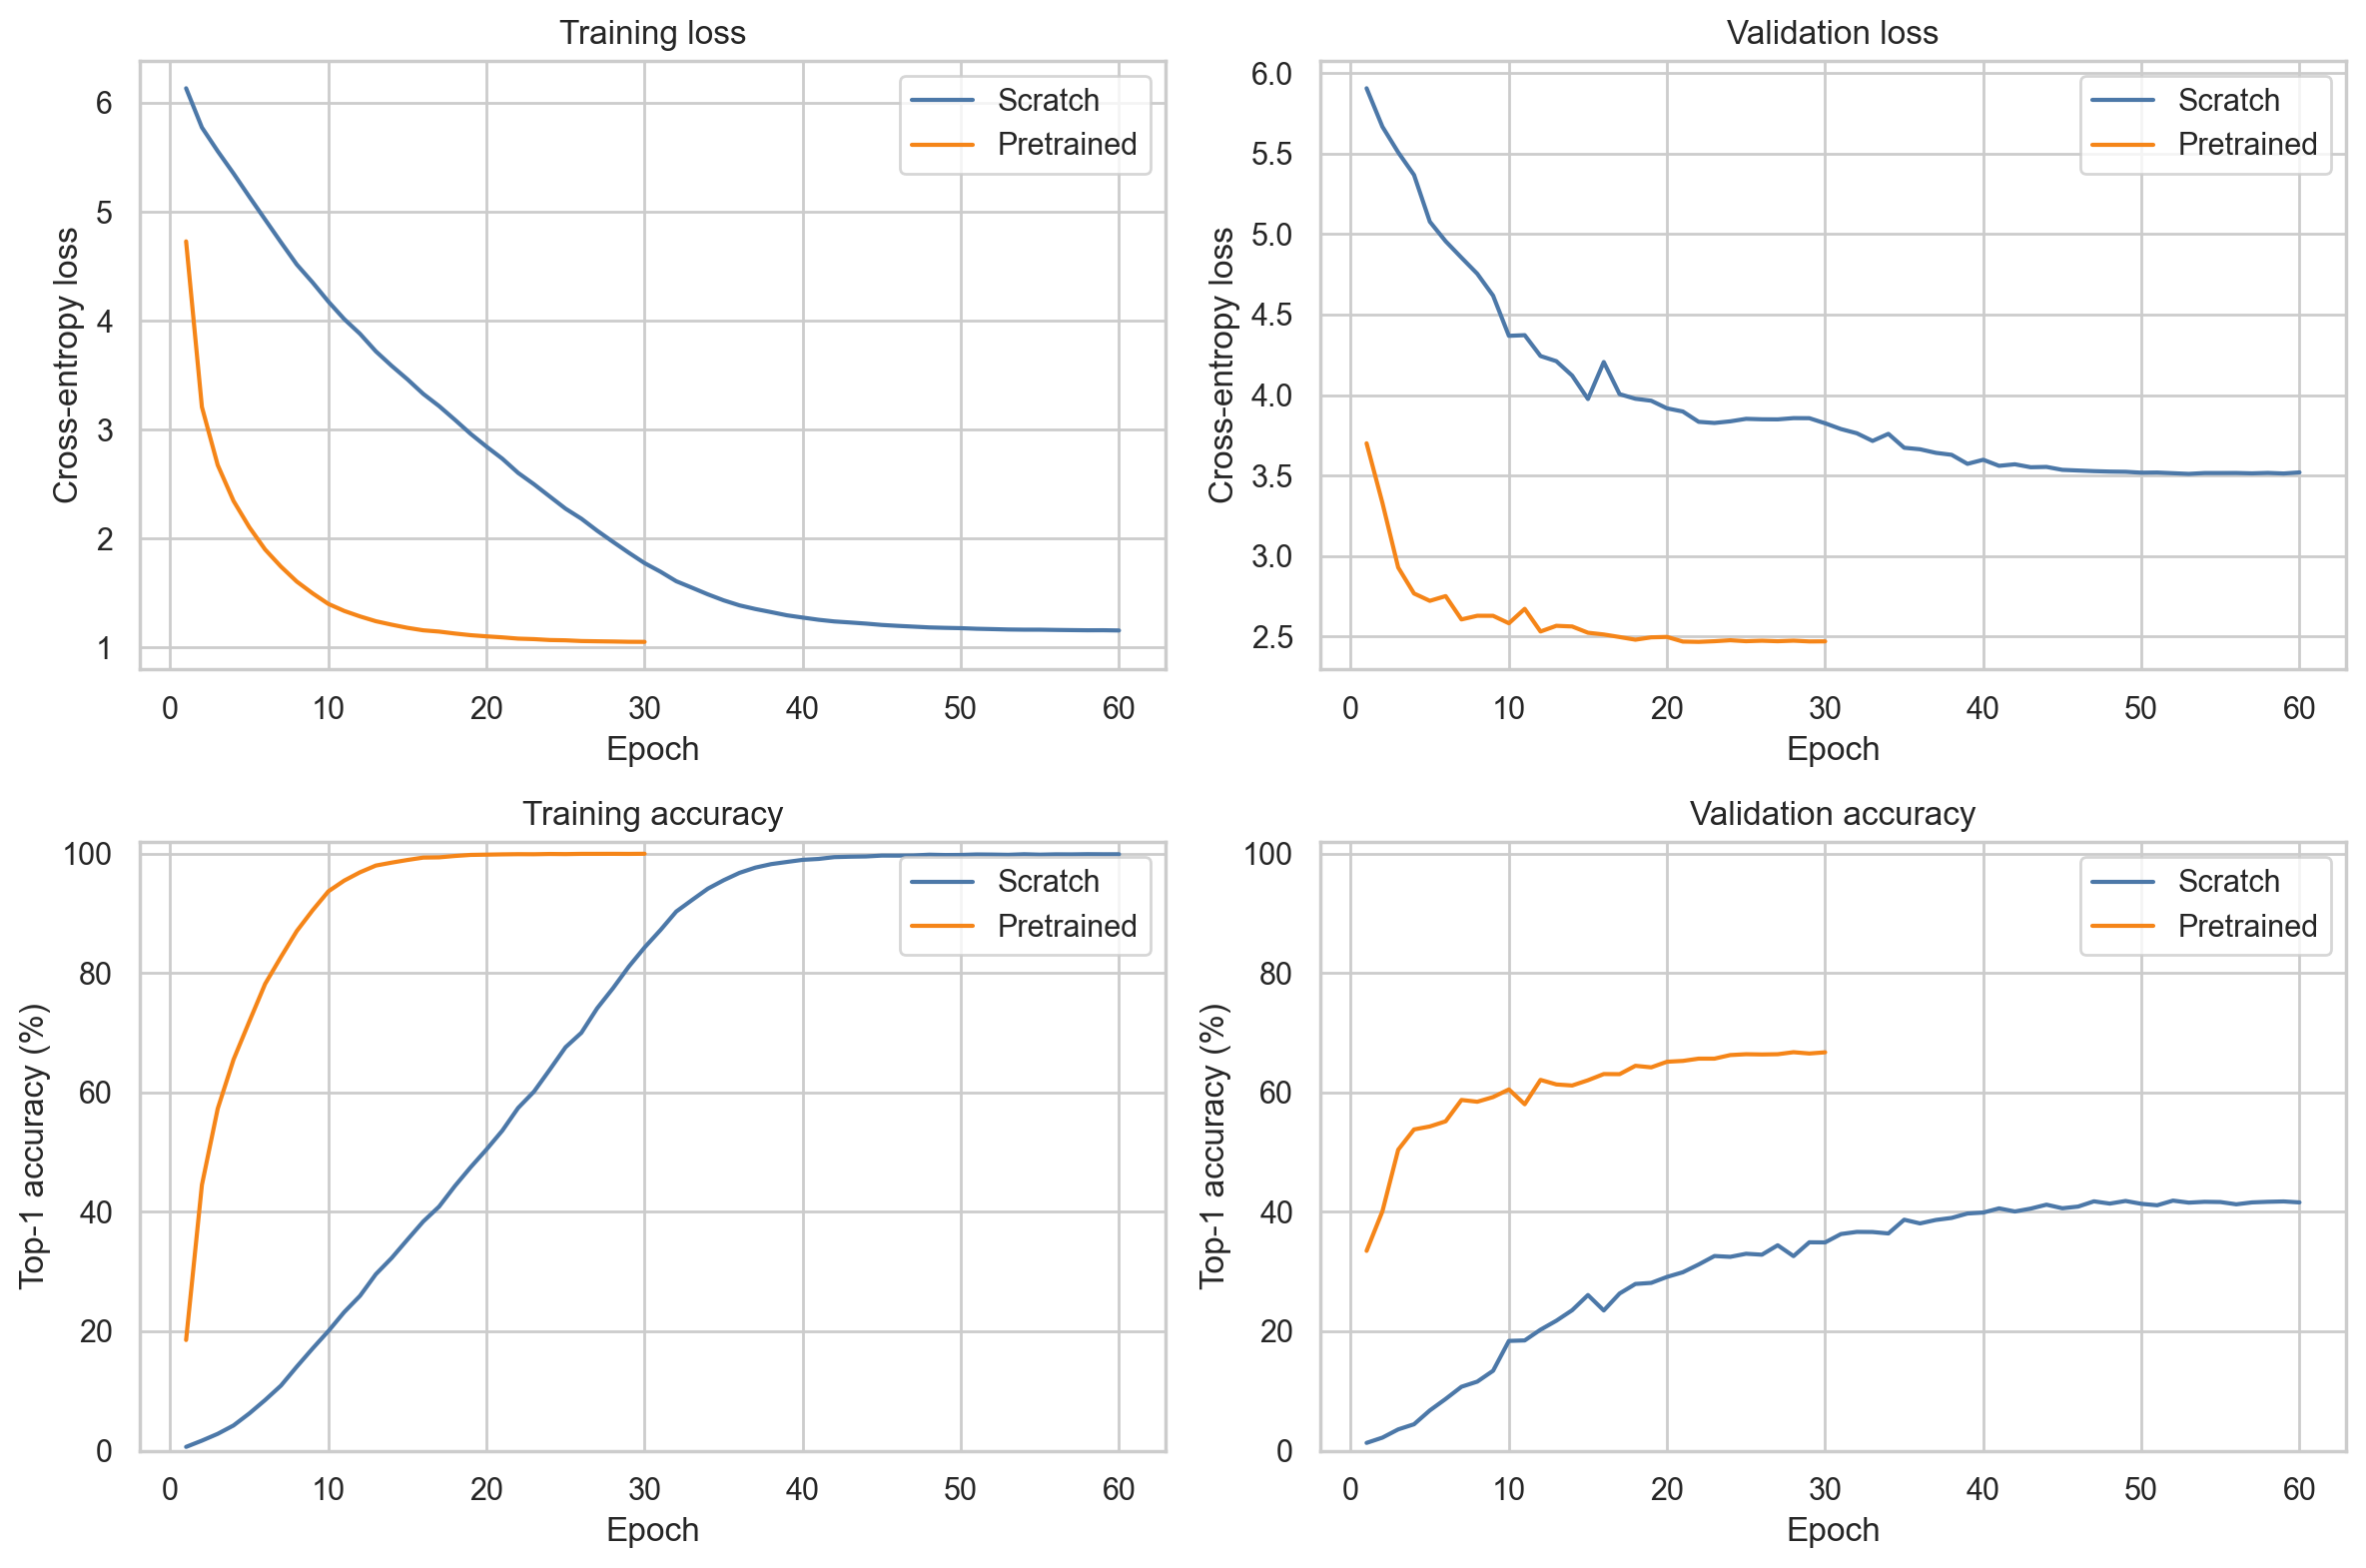
\includegraphics[width=0.96\textwidth]{figures/learning_curves_comparison.png}
    \caption{Training dynamics for the two ResNet-18 experiments.  ImageNet initialisation begins at much higher accuracy and converges rapidly, but both runs ultimately exhibit a large train--validation gap.}
    \label{fig:curves}
\end{figure*}

\subsection{Convergence and generalisation}
Figure~\ref{fig:curves} makes the benefit of transfer learning clear.  Validation top-1 goes above 50\% in the first few epochs for the pretrained model.  The scratch model takes about 30 epochs to get close to 40\%.  The best pretrained checkpoint is epoch 22, while the scratch model reaches its best checkpoint at epoch 53.  The recorded MPS training time up to these checkpoints was 5,633~s (1.56~h) and 13,550~s (3.76~h), respectively.

Both models reach almost 100\% training accuracy, but validation and test accuracy stop near 66\% for pretraining and 42\% for scratch.  The loss curves also separate, so this is overfitting and not just random accuracy fluctuation.  Augmentation, label smoothing, weight decay, cosine scheduling, and saving the best validation checkpoint help, but they do not fully solve it.  With 500 classes and only 40 training images per class, training for more epochs alone is not a good solution.

\subsection{Traditional feature ablations}
The HOG/HSV runs show that combining features does not automatically improve the result.  HOG gets 1.78\% macro-F1, HSV gets 1.58\%, and HOG+HSV gets 1.67\%.  For larger $C$, HOG gets a very high training score but stays near 2\% validation macro-F1.  So it is mostly memorising the training set.  HSV is fast and small, but loses spatial information.  HOG has shape information, but it is not as flexible as local SIFT matching when species images have different poses and backgrounds.

\begin{figure}[t]
    \centering
    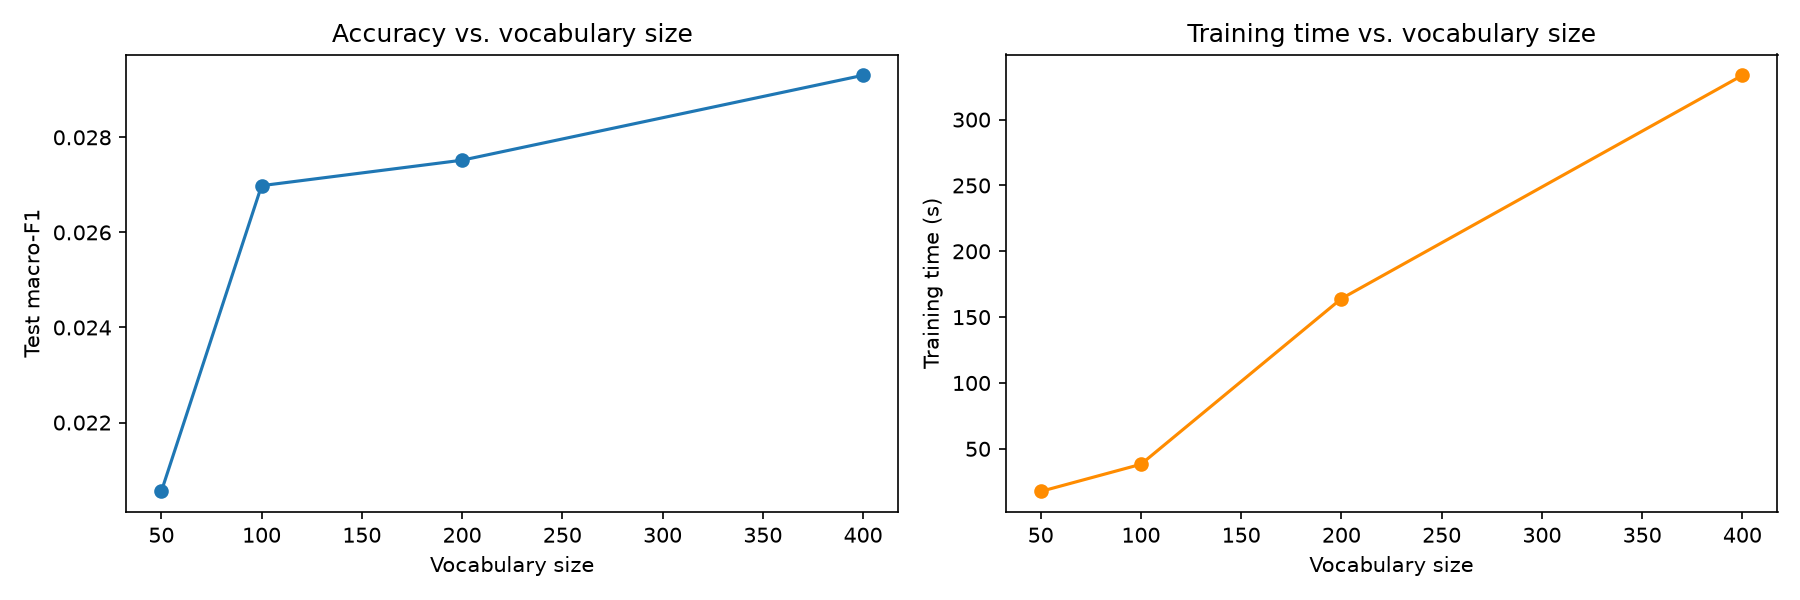
\includegraphics[width=\linewidth]{figures/vocab_size_ablation.png}
    \caption{SIFT--BoVW vocabulary ablation.  Larger vocabularies cost substantially more to fit; test macro-F1 rises only modestly.}
    \label{fig:vocab}
\end{figure}

For SIFT--BoVW, changing vocabulary size gives an accuracy versus time trade-off (Figure~\ref{fig:vocab}).  Table~\ref{tab:vocab} shows that $K=100$ has the best validation macro-F1 (3.13\%).  $K=400$ has the best test top-1 (3.86\%) and test macro-F1 (2.93\%), but takes 333.6~s to fit.  We report $K=200$ as a middle setting.  It is important to note that it is not the best validation setting, so we are not selecting the result after looking at the test set.

\begin{table}[t]
\centering
\caption{SIFT vocabulary ablation.  F1 and top-1 are percentages; time is classifier fit time.}
\label{tab:vocab}
\small
\begin{tabular}{rrrrr}
\toprule
$K$ & Val F1 & Test F1 & Top-1 & Fit (s) \\
\midrule
50  & 2.57 & 2.05 & 2.58 & 17.7 \\
100 & \textbf{3.13} & 2.70 & 3.34 & 38.3 \\
200 & 3.11 & 2.75 & 3.42 & 164.1 \\
400 & 3.00 & \textbf{2.93} & \textbf{3.86} & 333.6 \\
\bottomrule
\end{tabular}
\end{table}

Classifier choice also changes the result.  On $K=200$ features, the linear SGD classifier is better than random forest by 1.38 top-1 points and 1.15 macro-F1 points.  It also fits in 169.6~s instead of 391.6~s.  The SIFT histograms are large and sparse, so a linear classifier seems to work better than the depth-limited forest in this case.

\subsection{Efficiency and timing scope}
The deep models process about 218 test images/s in the recorded inference loop.  The saved traditional prediction times look much smaller (16~ms for 5,000 SIFT histograms and 9.5~ms for HSV), but these numbers only time classifier prediction after features are already computed.  They do not include SIFT detection, visual-word assignment, HOG/HSV extraction, file reading, or cache creation.  So the classical and deep throughput numbers are not a fair end-to-end comparison.  For the HOG/HSV experiment, extraction for all splits takes 42.1~s for HSV, 66.3~s for HOG, and 88.0~s for HOG+HSV.  Hyperparameter search adds 10.5, 768.4, and 843.4~s.  The useful takeaway is that a cached linear classifier is fast to try again, not that the full SIFT system is thousands of times faster than a CNN.

\section{Error and Interpretability Analysis}
\subsection{Traditional successes and failures}
Figure~\ref{fig:examples} shows some correct and wrong SIFT predictions.  The correct ones often have a large, clear object in the centre.  Wrong predictions are common when the subject is small, the background is busy, or the image has an unusual viewpoint.  Some errors are between visually similar species, which means SIFT captures some broad shape and texture.  Other errors are between very different groups.  This is one weakness of BoVW: after keypoints are pooled into one histogram, the original layout information is lost.

\begin{figure*}[t]
\centering
\begin{minipage}{0.49\textwidth}
  \centering
  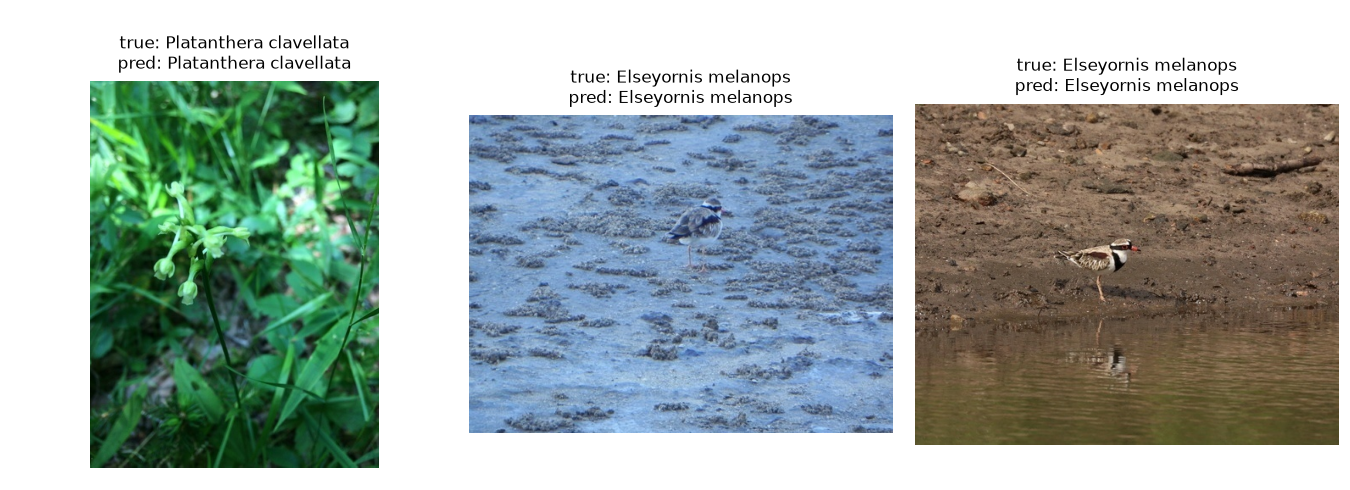
\includegraphics[width=\linewidth]{figures/examples_correct_excerpt.png}
  \centerline{(a) Correct SIFT--BoVW predictions}
\end{minipage}\hfill
\begin{minipage}{0.49\textwidth}
  \centering
  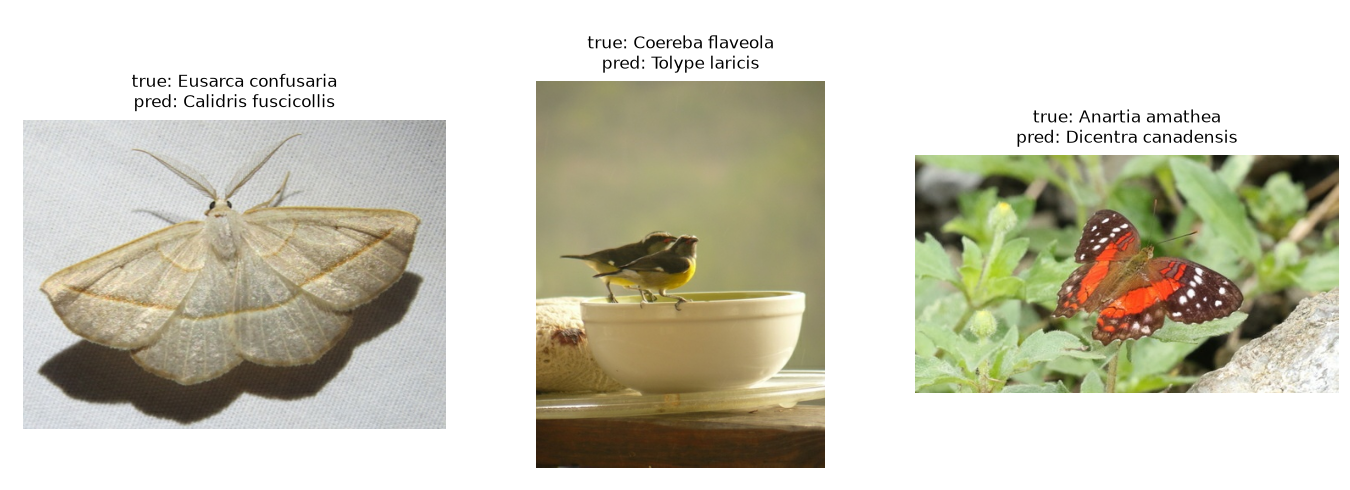
\includegraphics[width=\linewidth]{figures/examples_incorrect_excerpt.png}
  \centerline{(b) Incorrect SIFT--BoVW predictions}
\end{minipage}
\caption{Selected successful and failed examples from the primary traditional method.  Labels identify the true and predicted species; the repository artifacts retain six examples in each category.}
\label{fig:examples}
\end{figure*}

\subsection{Confusion structure}
The repository also saves full 500-class confusion matrices and the most common confusion pairs.  Figure~\ref{fig:confusion} shows a readable 15-class SIFT subset.  The diagonal is weak because SIFT top-1 is only 3.42\%, but some off-diagonal cells repeat more than others, so the errors are not fully random.  For the neural models, pretraining improves many classes, but hard pairs still remain.  The pretrained top-5 score is 17.28 points higher than top-1, which means the correct species is often among the likely predictions but not ranked first.

\begin{figure}[t]
    \centering
    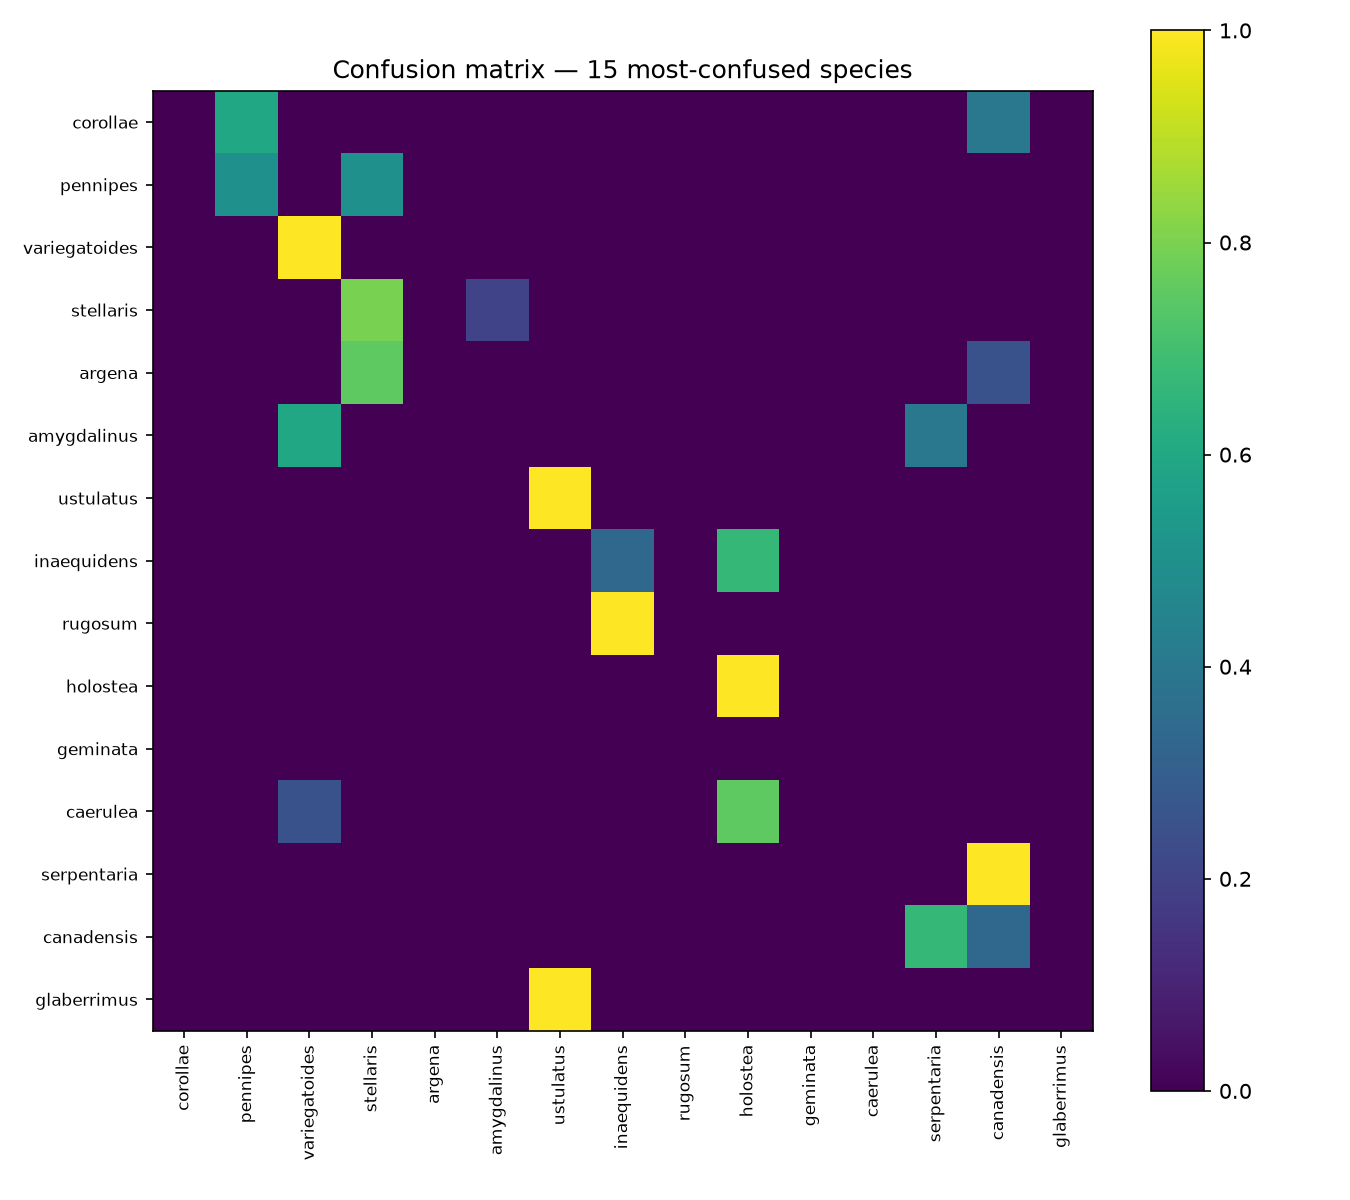
\includegraphics[width=0.98\linewidth]{figures/confusion_matrix_subset.png}
    \caption{Normalised confusion matrix for a 15-class subset of the SIFT--BoVW test predictions.}
    \label{fig:confusion}
\end{figure}

\subsection{Grad-CAM case study}
The most common directed confusion in the saved scratch-model analysis is \emph{Lupinus perennis} predicted as \emph{Agastache foeniculum}.  In Figure~\ref{fig:gradcam}, Grad-CAM mostly highlights the flower spike and nearby plant region.  So the model is often looking at the relevant object, but it still cannot separate these similar plants properly.  In some other wrong cases, the attention also covers the background or a central region.  This suggests that we need both better fine-grained features and better localisation, not only background removal.

\begin{figure}[t]
    \centering
    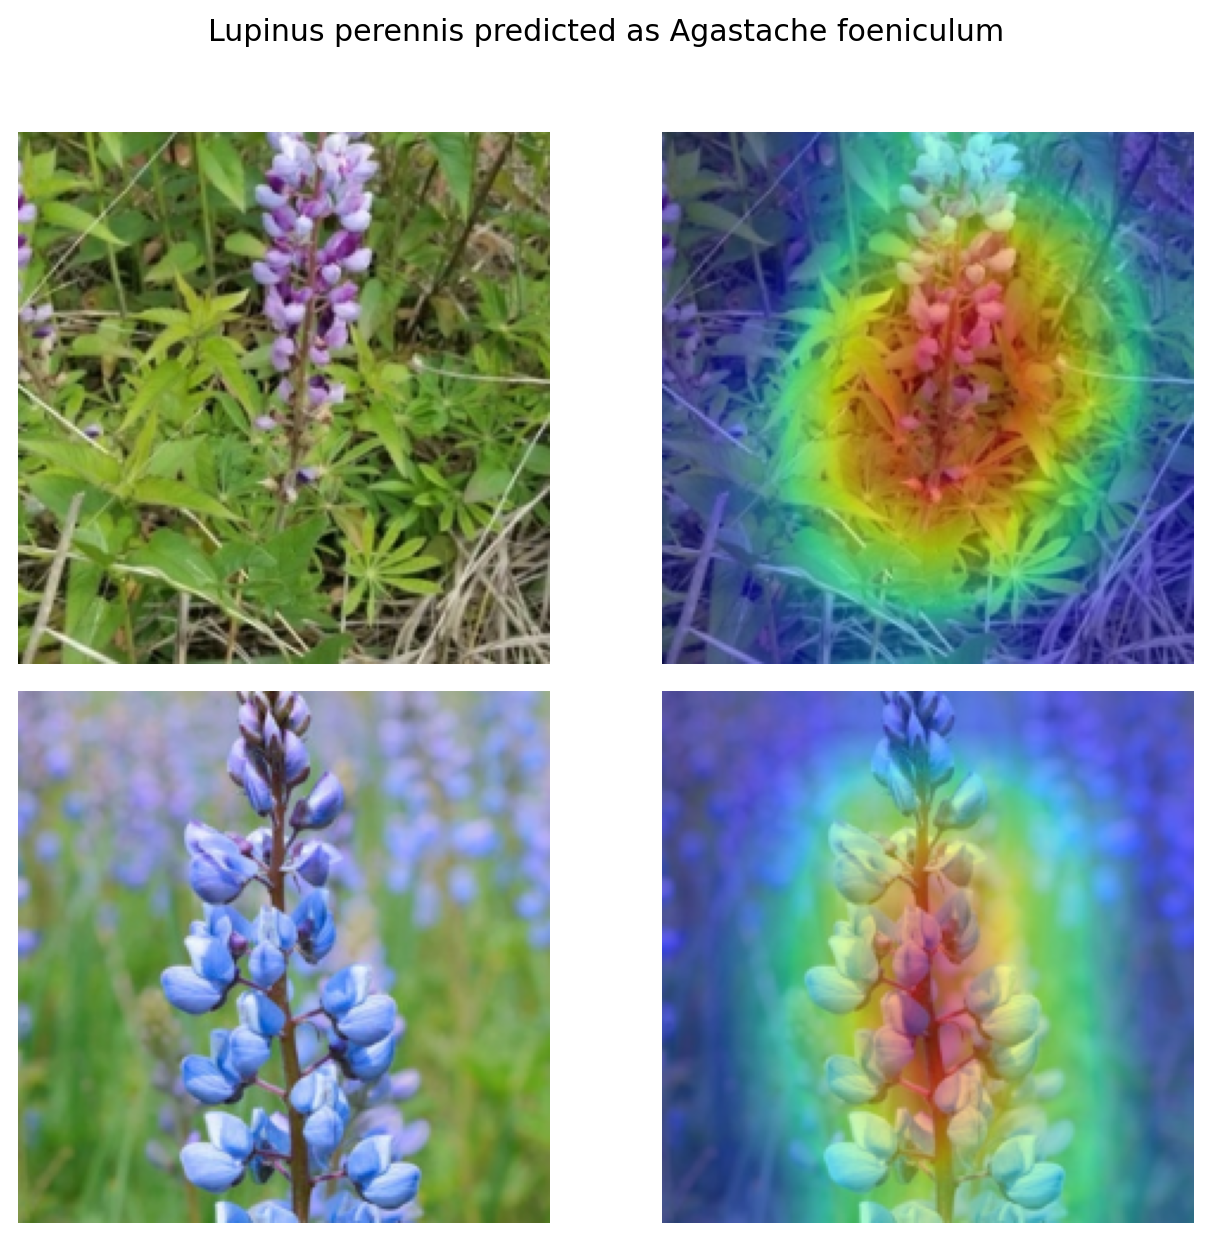
\includegraphics[width=\linewidth]{figures/gradcam_confused_pair_excerpt.png}
    \caption{Representative Grad-CAM examples from the largest directed confusion pair of the scratch ResNet-18.  Each row contains an input and its overlay; the maps cover the plant/flower structure despite the wrong species prediction.  The repository artifact contains five such pairs; two are shown here at readable scale.}
    \label{fig:gradcam}
\end{figure}

\section{Discussion}
The overall result is quite clear.  Classical features do better than random guessing, but they are not enough for 500-way species recognition.  HSV loses location information, HOG uses a fixed grid, and BoVW loses the position of SIFT keypoints.  Training a bigger classical classifier did not fix this: random forest was worse than the linear SGD model.  CNNs learn spatial features from the data and give a much larger improvement.  ImageNet pretraining helps the most because the model does not have to learn basic visual features only from 40 images per class.

The best top-1 accuracy is 66.02\%, which is good for our first full pipeline but still leaves a lot of room.  Training accuracy is close to 100\% while validation accuracy stays near 66\%, so just running more epochs is unlikely to push it to 80\%.  Next, we would try stronger but sensible augmentation such as RandAugment or MixUp/CutMix, a stronger pretrained backbone, higher image resolution, and methods that focus on confusing species pairs.  If genus or family labels can be added without touching the test set, hierarchy-aware training could also help.

There are a few limitations in our comparison.  The scratch and pretrained runs use different optimisers, so the result compares the full practical training setups, not only the initial weights.  A better controlled experiment would keep the optimiser and schedule the same.  Also, the saved classical timing does not include feature extraction, so it should not be compared directly with the CNN timing.  We only generated Grad-CAM results for the scratch model.  Finally, our 500-species subset is balanced, while the original iNaturalist data is long-tailed.  Therefore, these results do not directly show how well the methods handle real class imbalance.

\section{Reproducibility and Repository Coverage}
The repository has notebooks \texttt{00} to \texttt{05} for data preparation, scratch ResNet, pretrained ResNet, Grad-CAM, model comparison, and the two traditional methods (HOG/HSV and SIFT--BoVW).  Shared Python code handles data loading, model creation, training, checkpoints, metrics, plots, handcrafted features, and Grad-CAM.  YAML files store the deep-learning settings and the HOG/HSV search values.  Each experiment saves JSON/CSV files and figures under \texttt{results/}, and the comparison notebook reads these saved outputs.  Checkpoints and the image archive are not in Git because they are too large.

All experiments use seed 42 and the same class mapping.  To rerun the project, first prepare and validate the dataset manifests, then run each method notebook, followed by the comparison and Grad-CAM notebooks.  The tests cover configuration loading, data transforms and manifests, model shapes, evaluation, Grad-CAM utilities, and classical feature helpers.  Keeping settings, source code, notebooks, and saved results separate makes the project easier to follow and reproduce.

\section{Conclusion}
In this project, we compared classical image features and ResNet-18 models for 500-species iNaturalist classification.  SIFT--BoVW was the best classical method, but it reached only 3.42\% top-1.  ResNet-18 from scratch reached 41.98\%, and ImageNet fine-tuning reached 66.02\% top-1 and 83.30\% top-5.  So transfer learning was clearly the most useful thing we tried.  HOG/HSV features, BoVW pooling, random forest, and longer scratch training did not solve the fine-grained classification problem.  The learning curves show overfitting, and the error examples show that similar species are still difficult.  Our next steps would be better pretrained models, higher resolution or part-aware models, stronger controlled augmentation, and experiments designed for hard species pairs.

{\small
\bibliographystyle{ieeenat_fullname}
\bibliography{references}
}

\end{document}
